\chapter{Specifikacija programske potpore}
		
	\section{Funkcionalni zahtjevi}
			
			\noindent \textbf{Dionici:}
			
			\begin{packed_enum}
				
				\item Vlasnik (naručitelj)				
				\item Zaposlenici šahovskog kluba
				\begin{packed_enum}
						
					\item Treneri
						
				\end{packed_enum}
				\item Članovi šahovskog kluba
				\item Neregistrirani korisnici aplikacije
				\item Administrator
				\item Razvojni tim
				
			\end{packed_enum}
			
			\noindent \textbf{Aktori i njihovi funkcionalni zahtjevi:}
			
			
			\begin{packed_enum}
				\item  \underbar{Trener (inicijator) može:}
				
				\begin{packed_enum}
					
					\item prijaviti se u aplikaciju putem korisničkog imena i lozinke
					\item odjaviti se iz aplikacije
					\item postavljati dnevne šahovske taktike
					\item revidirati prijavljene pogrešne taktike
					\item slagati raspored vlastitih treninga
					\item organizirati turnire
					\item vidjeti rang liste članova
					\item pristupiti i objavljivati novi sadržaj na stranici novosti 
					\item vidjeti osobne podatke i aktivnosti svojeg profila
					
				\end{packed_enum}
			
				\item  \underbar{Član šahovskog kluba (inicijator) može:}
				
				\begin{packed_enum}
					
					\item prijaviti se u aplikaciju putem korisničkog imena i lozinke
					\item odjaviti se iz aplikacije
					\item platiti članarinu putem aplikacije
					\item prijavljivati se na treninge kod pojedinih trenera
					\item prijavljivati se na turnire
					\item rješavati dnevne šahovske taktike
					\begin{packed_enum}
						
						\item nakon rješavanja dnevne šahovske taktike mogu joj dodijeliti ocjenu
						\item nakon rješavanja dnevne šahovske taktike mogu prijaviti grešku u taktici
						
					\end{packed_enum}
					\item vidjeti rang liste članova
					\item pristupiti stranici novosti
					\item vidjeti osobne podatke i aktivnosti svojeg profila
					
				\end{packed_enum}
			
				\item \underbar{Administrator (inicijator) može:}
				
				\begin{packed_enum}
					
					\item prijaviti se u aplikaciju putem korisničkog imena i lozinke
					\item odjaviti se iz aplikacije
					\item potpuno zabraniti pristup bilo kojem članu ili treneru
					\item zabraniti pristup bilo čemu \textbf{osim} uplate članarine bilo kojem članu
					\item vidjeti rang liste članova
					\item objavljivati i skidati sadržaj na stranici novosti
					\item mijenjati raspored treninga bilo kojem treneru
					\item postavljati i skidati dnevne šahovske taktike
					\begin{packed_enum}
						
						\item nakon rješavanja dnevne šahovske taktike mogu joj dodijeliti ocjenu
						\item nakon rješavanja dnevne šahovske taktike mogu prijaviti grešku u taktici
						
					\end{packed_enum}
					\item dodavati i skidati turnire
					\item pregledavati transakcije
					\item vidjeti osobne podatke i aktivnosti svojeg profila
					
				\end{packed_enum}
			
				\item \underbar{Neregistrirani korisnik (inicijator) može:}
				
				\begin{packed_enum}
					
					\item registrirati se
					\item rješavati dnevne šahovske taktike
					\item vidjeti rang liste članova
					\item pristupiti novostima
					
				\end{packed_enum}
			
				\item \underbar{Baza podataka (sudionik):}
				
				\begin{packed_enum}
					
					\item pohranjuje sve podatke o korisnicima i njihovim ovlastima
					\item pohranjuje sve dnevne šahovske taktike
					\item pohranjuje rang listu članova
					\item pohranjuje povijest svih transakcija
					\item pohranjuje termine svih treninga
					\item pohranjuje termine svih turnira
					\item pohranjuje svaku stavku na stranici novosti
					
				\end{packed_enum}
				
			\end{packed_enum}
			
			\eject 
			
			
				
			\subsection{Obrasci uporabe}
				
				\subsubsection{Opis obrazaca uporabe}
					
					\noindent \underbar{\textbf{UC1 - Registracija}}
					\begin{packed_item}
	
						\item \textbf{Glavni sudionik: } Neregistrirani korisnik
						\item  \textbf{Cilj: } Stvoriti korisnički račun za pristup sustavu
						\item  \textbf{Sudionici: } Baza podataka
						\item  \textbf{Preduvjet: } -
						\item  \textbf{Opis osnovnog tijeka:}
						
						\item[] \begin{packed_enum}
	
							\item Korisnik otvara sučelje za registraciju
							\item Korisnik unosi sve potrebne podatke za registraciju
							\item Korisnik prima obavijest o uspješnosti registracije
							
						\end{packed_enum}
						
						\item  \textbf{Opis mogućih odstupanja:}
						
						\item[] \begin{packed_item}
	
							\item[2.a] Unos već postojećeg korisničkog imena i/ili e-maila, unos nepostojećeg e-maila, unos podatka u nedozvoljenom formatu.
							\item[] \begin{packed_enum}
								
								\item Sučelje obavještava korisnika o pogrešci u registraciji i vraća ga na stranicu za registraciju.
								\item Korisnik mijenja podatke i pokušava ponovo ili odustaje od registracije.
								
							\end{packed_enum}
							
						\end{packed_item}
					\end{packed_item}
					

					\noindent \underbar{\textbf{UC2 - Pregled dnevnih taktika}}
					\begin{packed_item}
	
						\item \textbf{Glavni sudionik: } Neregistrirani korisnik, član, administrator
						\item  \textbf{Cilj: } Pregledati dostupne taktike za rješavanje tog dana
						\item  \textbf{Sudionici: } Baza podataka
						\item  \textbf{Preduvjet: } -
						\item  \textbf{Opis osnovnog tijeka:}
						
						\item[] \begin{packed_enum}
	
							\item Korisnik otvara stranicu s popisom dnevnih taktika
							\item Korisnik odabire taktiku koju želi rješavati
							\item Pokreće se simulacija šahovske ploče s odabranom taktikom
							
						\end{packed_enum}
					\end{packed_item}
			


					\noindent \underbar{\textbf{UC3 - Rješavanje dnevne taktike}}
					\begin{packed_item}
	
						\item \textbf{Glavni sudionik: } Neregistrirani korisnik, član, administrator
						\item  \textbf{Cilj: } Uspješno riješiti odabranu dnevnu taktiku
						\item  \textbf{Sudionici: }-
						\item  \textbf{Preduvjet: }-
						\item  \textbf{Opis osnovnog tijeka:}
						
						\item[] \begin{packed_enum}
	
							\item Korisniku se pokreće simulacija šahovske ploče
							\item Korisnik rješava dnevnu taktiku
							\item Simulacija se zatvara po uspješnom rješavanju
							
						\end{packed_enum}
						
						\item  \textbf{Opis mogućih odstupanja:}
						
						\item[] \begin{packed_item}
	
							
							\item[2.a] Korisnik napravi pogrešan potez
							\item[] \begin{packed_enum}
								
								\item Simulacija obavještava korisnika o pogrešnom potezu i vraća ploču u stanje prije pogrešnog poteza.
								\item Korisnik pokušava s novim potezom.
								
								
							\end{packed_enum}
						
						\item[3.a] Korisnik želi ocijeniti dnevnu taktiku
						\item[] \begin{packed_enum}
							
							\item Korisnik odabire opciju "Unesi ocjenu"
							\item Korisnik potvrđuje odabranu ocjenu ili odustaje od davanja ocjene
							
						\end{packed_enum}
					
						\item[3.b] Korisnik želi prijaviti pogrešku u taktici
					\item[] \begin{packed_enum}
						
						\item Član odabire opciju "Prijavi pogrešku u taktici"
						\item Korisnik unosi nove poteze i opis novih poteza
						\item Korisnik potvrđuje unesene informacije ili odustaje od unosa novih poteza i njihovih opisa
							\end{packed_enum}
						\end{packed_item}
					\end{packed_item}
					

					\noindent \underbar{\textbf{UC4 - Pregled rang liste}}
					\begin{packed_item}
	
						\item \textbf{Glavni sudionik: }Korisnik, član, trener, administrator
						\item  \textbf{Cilj: }Pregledati rang listu članova kluba
						\item  \textbf{Sudionici: }Baza podataka
						\item  \textbf{Preduvjet: }Ako je korisnik prijavljen kao član mora imati tekuću članarinu
						\item  \textbf{Opis osnovnog tijeka:}
						
						\item[] \begin{packed_enum}
	
							\item Korisnik otvara stranicu s rang listom
							\item Prikazuje se rang lista članova kluba
							
						\end{packed_enum}
					\end{packed_item}
				
					
					\noindent \underbar{\textbf{UC5 - Odjava}}
					\begin{packed_item}
	
						\item \textbf{Glavni sudionik: } Administrator, član, trener
						\item  \textbf{Cilj: } Okončati aktivnu sjednicu
						\item  \textbf{Sudionici: } Baza podataka
						\item  \textbf{Preduvjet: } -
						\item  \textbf{Opis osnovnog tijeka:}
						
						\item[] \begin{packed_enum}
	
							\item Klik na gumb 'Odjavi se'
							\item Učitavanje stranice novosti 
							
						\end{packed_enum}
					\end{packed_item}
				
				\vspace{\baselineskip}
				
					
					\noindent \underbar{\textbf{UC6 - Objava dnevne šahovske taktike}}
					\begin{packed_item}
	
						\item \textbf{Glavni sudionik: }Trener, administrator
						\item  \textbf{Cilj: } Stvoriti novu dnevnu šahovsku taktiku
						\item  \textbf{Sudionici: } Baza podataka
						\item  \textbf{Preduvjet: } -
						\item  \textbf{Opis osnovnog tijeka:}
						
						\item[] \begin{packed_enum}
	
							\item Otvaranje stranice za unos nove taktike
							\item Trener unosi podatke o taktici poput imena, težine itd.
							\item Trener namješta inicijalnu konfiguraciju ploče na interaktivnoj simulaciji
							\item Trener potvrđuje inicijalnu konfiguraciju
							\item Trener naizmjence pomiče crne i bijele šahovske figurice i tako unosi poteze taktike
							\item Trener potvrđuje korektan unos poteza i objavljuje dnevnu taktiku
							
						\end{packed_enum}
						
						\item  \textbf{Opis mogućih odstupanja:}
						
						\item[] \begin{packed_item}
	
							\item[3.a] Zabuna u namještanju inicijalne konfiguracije ploče
							\item[] \begin{packed_enum}
								
								\item klik na gumb 'reset'
								\item ploča se vraća na startnu konfiguraciju
								
							\end{packed_enum}
							
							\item[5.a] Zabuna u unosu poteza taktike
							\item[] \begin{packed_enum}
								
								\item klik na gumb 'reset'
								\item ploča se vraća na inicijalnu konfiguraciju unesenu u prošlom koraku
								
							\end{packed_enum}
							
						\end{packed_item}
					\end{packed_item}
					
					\noindent \underbar{\textbf{UC7 - Pregled vlastitih treninga}}
					\begin{packed_item}
	
						\item \textbf{Glavni sudionik: }Trener
						\item  \textbf{Cilj: } Prikazati sve buduće treninge prijavljenog trenera
						\item  \textbf{Sudionici: } Baza podataka
						\item  \textbf{Preduvjet: } -
						\item  \textbf{Opis osnovnog tijeka:}
						
						\item[] \begin{packed_enum}
	
							\item Klik na karticu 'Treninzi'
							\item Kronološki prikaz svih budućih treninga 
						\end{packed_enum}
					\end{packed_item}
					
					
					\noindent \underbar{\textbf{UC8 - Brisanje treninga}}
					\begin{packed_item}
	
						\item \textbf{Glavni sudionik: }Trener, Administrator
						\item  \textbf{Cilj: } Obrisati postojeći trening
						\item  \textbf{Sudionici: } Baza podataka
						\item  \textbf{Preduvjet: } -
						\item  \textbf{Opis osnovnog tijeka:}
						
						\item[] \begin{packed_enum}
	
							\item klik na gumb za brisanje jednog od prikazanih treninga
							\item prikaz dijaloškog okvira koji traži potvrdu od korisnika da uistinu želi obrisati trening
							\item nakon davanja potvrde trening nestaje iz prikaza
							
						\end{packed_enum}
						
						\item  \textbf{Opis mogućih odstupanja:}
						
						\item[] \begin{packed_item}
	
							\item[3.a] Korisnik se predomisli o brisanju treninga
							\item[] \begin{packed_enum}
								
								\item pritisak na gumb 'odustani' u dijaloškom okviru za potvrdu
								
							\end{packed_enum}
							
						\end{packed_item}
					\end{packed_item}
					
					
					\noindent \underbar{\textbf{UC9 - Stvaranje novog treninga}}
					\begin{packed_item}
	
						\item \textbf{Glavni sudionik: }Trener, Administrator
						\item  \textbf{Cilj: } Stvoriti novi trening
						\item  \textbf{Sudionici: } Baza podataka
						\item  \textbf{Preduvjet: } -
						\item  \textbf{Opis osnovnog tijeka:}
						
						\item[] \begin{packed_enum}
	
							\item klik na gumb za dodavanje novog treninga
							\item prikaz dijaloškog okvira u koji korisnik unosi podatke o treningu kao vrijeme, naziv, izvoditelj itd.
							\item klik na gumb za stvaranje treninga
							\item zatvara se dijaloški okvir i novi trening dodaje se u prikaz treninga
							
						\end{packed_enum}
						
						\item  \textbf{Opis mogućih odstupanja:}
						
						\item[] \begin{packed_item}
	
							\item[2.a]Trener dodaj podatke
							\item[] \begin{packed_enum}
								
								\item trener ne može birati izvoditelja nego je on sam zaključan kao izvoditelj prilikom stvaranja
								
								
							\end{packed_enum}
						
						
							\item[3.a] Odustajanje od stvaranja novog treninga
							\item[] \begin{packed_enum}
								
								\item pritisak na gumb 'odustani' u dijaloškom okviru za unos podataka o treningu
								\item zatvaranje dijaloškog okvira i odbacivanje unesenih podataka
								
							\end{packed_enum}
						
						
							
						\end{packed_item}
					\end{packed_item}
				
					
					\noindent \underbar{\textbf{UC10 - Pregled turnira}}
					\begin{packed_item}
	
						\item \textbf{Glavni sudionik: }Trener, administrator, član
						\item  \textbf{Cilj: } Prikazati sve buduće turnire
						\item  \textbf{Sudionici: } Baza podataka
						\item  \textbf{Preduvjet: } -
						\item  \textbf{Opis osnovnog tijeka:}
						
						\item[] \begin{packed_enum}
	
							\item Klik na karticu 'Turniri'
							\item Kronološki prikaz svih budućih turnira
						\end{packed_enum}
					\end{packed_item}
					
					\noindent \underbar{\textbf{UC11 - Brisanje turnira}}
					\begin{packed_item}
	
						\item \textbf{Glavni sudionik: }Trener, administrator
						\item  \textbf{Cilj: } Obrisati postojeći turnir čiji je organizator prijavljeni korisnik
						\item  \textbf{Sudionici: } Baza podataka
						\item  \textbf{Preduvjet: } Ako je korisnik prijavljen kao trener, može brisati samo svoje turnire
						\item  \textbf{Opis osnovnog tijeka:}
						
						\item[] \begin{packed_enum}
	
							\item klik na gumb za brisanje jednog od prikazanih turnira
							\item prikaz dijaloškog okvira koji traži potvrdu od korisnika da uistinu želi obrisati turnir
							\item nakon davanja potvrde turnir nestaje iz prikaza
							
						\end{packed_enum}
						
						\item  \textbf{Opis mogućih odstupanja:}
						
						\item[] \begin{packed_item}
	
							\item[3.a] Korisnik se predomisli o brisanju turnira
							\item[] \begin{packed_enum}
								
								\item pritisak na gumb 'odustani' u dijaloškom okviru za potvrdu
								
							\end{packed_enum}
							
						\end{packed_item}
					\end{packed_item}
				
					
					\noindent \underbar{\textbf{UC12 - Stvaranje novog turnira}}
					\begin{packed_item}
	
						\item \textbf{Glavni sudionik: }Trener, administrator
						\item  \textbf{Cilj: } Stvoriti novi turnir
						\item  \textbf{Sudionici: } Baza podataka
						\item  \textbf{Preduvjet: } Korisnik se nalazi na stranici pregleda turnira
						\item  \textbf{Opis osnovnog tijeka:}
						
						\item[] \begin{packed_enum}
	
							\item klik na gumb za dodavanje novog turnira
							\item prikaz dijaloškog okvira u koji korisnik unosi podatke o turniru kao vrijeme, naziv, izvoditelj itd.
							\item klik na gumb za stvaranje turnira
							\item zatvara se dijaloški okvir i novi turnir dodaje se na stranicu
							
						\end{packed_enum}
						
						\item  \textbf{Opis mogućih odstupanja:}
						
						\item[] \begin{packed_item}
							
							\item[2.a]Trener dodaj podatke
							\item[] \begin{packed_enum}
								
								\item trener ne može birati izvoditelja nego je on sam zaključan kao izvoditelj prilikom stvaranja
								
								
							\end{packed_enum}
						
						
							\item[3.a] Odustajanje od stvaranja novog turnira
							\item[] \begin{packed_enum}
								
								\item pritisak na gumb 'odustani' u dijaloškom okviru za unos podataka
								\item zatvaranje dijaloškog okvira i odbacivanje unesenih podataka
								
							\end{packed_enum}
							
						\end{packed_item}
					\end{packed_item}
					
					\noindent \underbar{\textbf{UC13 - Pristup stranici novosti}}
					\begin{packed_item}
	
						\item \textbf{Glavni sudionik: }Član, trener, administrator, neregistrirani korisnik
						\item  \textbf{Cilj: } Vidjeti sve nedavne novosti
						\item  \textbf{Sudionici: } Baza podataka
						\item  \textbf{Preduvjet: } -
						\item  \textbf{Opis osnovnog tijeka:}
						
						\item[] \begin{packed_enum}
	
							\item klik na karticu 'novosti'
							\item prikaz svih nedavnih novosti
							
						\end{packed_enum}
						
					\end{packed_item}
				
					
					\noindent \underbar{\textbf{UC14 - Objava novosti}}
					\begin{packed_item}
	
						\item \textbf{Glavni sudionik: }Trener, administrator
						\item  \textbf{Cilj: } Objaviti novost na stranici novosti
						\item  \textbf{Sudionici: } Baza podataka
						\item  \textbf{Preduvjet: } -
						\item  \textbf{Opis osnovnog tijeka:}
						
						\item[] \begin{packed_enum}
	
							\item klik na gumb za objavu novosti
							\item ispunjavanje dijaloškog okvira za stvaranje novosti
							\item klik na gumb za objavu
							\item novost se prikazuje na vrhu stranice novosti
							
						\end{packed_enum}
						
						\item  \textbf{Opis mogućih odstupanja:}
						
						\item[] \begin{packed_item}
	
							\item[3.a] Odustajanje od stvaranja novosti
							\item[] \begin{packed_enum}
								
								\item pritisak na gumb 'odustani' u dijaloškom okviru za unos podataka
								\item zatvaranje dijaloškog okvira i odbacivanje unesenih podataka
								
							\end{packed_enum}
							
						\end{packed_item}
					\end{packed_item}
					
					\noindent \underbar{\textbf{UC15 - Revidiranje pogreške u taktici}}
					\begin{packed_item}
	
						\item \textbf{Glavni sudionik: }Trener
						\item  \textbf{Cilj: } Prihvatiti ili odbaciti dojavu o pogrešci u nekoj taktici
						\item  \textbf{Sudionici: } Baza podataka
						\item  \textbf{Preduvjet: } Član je prijavio pogrešku u taktici
						\item  \textbf{Opis osnovnog tijeka:}
						
						\item[] \begin{packed_enum}
	
							\item otvara se pregled s detaljima o dojavi pogreške na taktici
							\item Trener klikom na gumb potvrđuje da je dojava o pogrešci valjana
							\item taktika u pitanju automatski se revidira te se ažuriraju i rang liste članova
							
						\end{packed_enum}
						
						\item  \textbf{Opis mogućih odstupanja:}
						
						\item[] \begin{packed_item}
	
							\item[2.a] Odbijanje dojave
							\item[] \begin{packed_enum}
								
								\item pritiskom na gumb 'odbaci' dojava se zanemaruje
								
							\end{packed_enum}
							
							
						\end{packed_item}
					\end{packed_item}
				
					
					\noindent \underbar{\textbf{UC16 - Pregled profila}}
					\begin{packed_item}
	
						\item \textbf{Glavni sudionik: }Administrator, član, trener
						\item  \textbf{Cilj: } pregled informacija vlastitog profila
						\item  \textbf{Sudionici: } Baza podataka
						\item  \textbf{Preduvjet: } -
						\item  \textbf{Opis osnovnog tijeka:}
						
						\item[] \begin{packed_enum}
	
							\item klik na karticu 'profil'
							\item učitava se prikaz osobnih podataka i svih aktivnosti na aplikaciji
							
						\end{packed_enum}
					\end{packed_item}
					

						\noindent \underbar{\textbf{UC17 - Prijava u korisnički račun}}
					\begin{packed_item}
						
						\item \textbf{Glavni sudionik: } Član, trener, administrator
						\item  \textbf{Cilj: } Prijaviti se u korisnički račun
						\item  \textbf{Sudionici: } Baza podataka
						\item  \textbf{Preduvjet: } -
						\item  \textbf{Opis osnovnog tijeka:}
						
						\item[] \begin{packed_enum}
							
							\item Korisnik otvara sučelje za prijavu u korisnički račun
							\item Korisnik upisuje korisničko ime i lozinku
							\item Korisniku se otvara stranica s novostima
							
						\end{packed_enum}
						
						\item  \textbf{Opis mogućih odstupanja:}
						
						\item[] \begin{packed_item}
							
							\item[3.a] Korisnik koji ima status člana nema plaćenu članarinu
							\item[] \begin{packed_enum}
								
								\item Korisniku se otvara stranica za uplatu članarine
								
							\end{packed_enum}
							
						\end{packed_item}
					\end{packed_item}
				
				
					\noindent \underbar{\textbf{UC18 - Uplata članarine}}
				\begin{packed_item}
					
					\item \textbf{Glavni sudionik: }Član
					\item  \textbf{Cilj: } Uplatiti članarinu
					\item  \textbf{Sudionici: } Baza podataka
					\item  \textbf{Preduvjet: } -
					\item  \textbf{Opis osnovnog tijeka:}
					
					\item[] \begin{packed_enum}
						
						\item Član odabire opciju "Uplata članarine"
						\item Članu se otvara sučelje s mogućnošću upisa potrebnih podataka za uplatu članarine  
						\item Član upisuje potrebne podatke za uplatu i potvrđuje svoj unos
						\item Član dobiva obavijest da je transakcija uspješna
						
					\end{packed_enum}
					
					\item  \textbf{Opis mogućih odstupanja:}
					
					\item[] \begin{packed_item}
						
					\item[3.a] Član je unio netočne podatke
					\item[] \begin{packed_enum}
						
						\item Članu dolazi obavijest o netočnom unosu podataka te mu se omogućuje da ponovno unese podatke
						
					\end{packed_enum}
						
					\end{packed_item}
				\end{packed_item}
			
			\noindent \underbar{\textbf{UC19 - Pregled dostupnih treninga}}
			\begin{packed_item}
				
				\item \textbf{Glavni sudionik: } Član
				\item  \textbf{Cilj: } Pregledati treninge na koje se može prijaviti
				\item  \textbf{Sudionici: } Baza podataka
				\item  \textbf{Preduvjet: } Član ima tekuću članarinu
				\item  \textbf{Opis osnovnog tijeka:}
				
				\item[] \begin{packed_enum}
					
					\item Član odabire opciju "Pregledaj treninge"
					\item Članu se prikazuje popis dostupnih treninga
					
				\end{packed_enum}
			\end{packed_item}
		
			
			\noindent \underbar{\textbf{UC20 - Prijava na trening}}
			\begin{packed_item}
				
				\item \textbf{Glavni sudionik: } Član
				\item  \textbf{Cilj: } Prijaviti se na trening kod odabranog trenera
				\item  \textbf{Sudionici: } Baza podataka
				\item  \textbf{Preduvjet: } Član ima tekuću članarinu
				\item  \textbf{Opis osnovnog tijeka:}
				
				\item[] \begin{packed_enum}
					
					\item Član odabire opciju "Prijavite trening"
					\item Članu se prikazuje popis raspoloživih trenera
					\item Član odabire jednog od ponuđenih trenera
					\item Član odabire jedan od raspoloživih termina treninga
					\item Član dobiva obavijest da je željeni termin treninga kod odabranog trenera zabilježen
					
				\end{packed_enum}
			\end{packed_item}
		
		\noindent \underbar{\textbf{UC21 - Prijava na turnir}}
		\begin{packed_item}
			
			\item \textbf{Glavni sudionik: } Član
			\item  \textbf{Cilj: } Prijaviti se na turnir
			\item  \textbf{Sudionici: } Baza podataka
			\item  \textbf{Preduvjet: } Član ima tekuću članarinu
			\item  \textbf{Opis osnovnog tijeka:}
			
			\item[] \begin{packed_enum}
				
				\item Član odabire opciju "Prijava na turnir"
				\item Članu se javlja obavijest o terminu sljedećeg turnira te poruka o nužnosti potvrde za prijavu na turnir uz mogućnost odabira opcije "Potvrđujem prijavu" ili opcije "Odustajem od prijave"
				\item Član odabire opciju "Potvrđujem prijavu"
				\item Član dobiva obavijest da je prijava zabilježena
				
			\end{packed_enum}
			
			\item  \textbf{Opis mogućih odstupanja:}
			
			\item[] \begin{packed_item}
				
				\item[2.a] Član odustaje od prijave
				\item[] \begin{packed_enum}
					
					\item Član odabire opciju "Odustajem od prijave"
					
				\end{packed_enum}
				
			\end{packed_item}
		\end{packed_item}
		
		
		\noindent \underbar{\textbf{UC22 - Brisanje novosti}}
		\begin{packed_item}
		
			\item \textbf{Glavni sudionik: } Administrator
			\item  \textbf{Cilj: } Obrisati novost sa stranice novosti
			\item  \textbf{Sudionici: } Baza podataka
			\item  \textbf{Preduvjet: } -
			\item  \textbf{Opis osnovnog tijeka:}
		
			\item[] \begin{packed_enum}
			
				\item Administrator se postavlja na listu novosti
				\item Administrator bira opciju "Obriši obavijest" pored obavijesti koju želi obrisati
				\item Administrator odabire opciju "Da" u dijaloškom okviru za potvrdu
			\end{packed_enum}
	
			\item  \textbf{Opis mogućih odstupanja:}
		
			\item[] \begin{packed_item}
			
				\item[3.a] Administrator odustaje od brisanja novosti
				\item[] \begin{packed_enum}
				
					\item Administrator odabire opciju "Ne" u dijaloškom okviru za potvrdu
				
				\end{packed_enum}
			\end{packed_item}
	
		\end{packed_item}

		\noindent \underbar{\textbf{UC23 - Zabrana pristupa treneru ili članu}}
		\begin{packed_item}
		
			\item \textbf{Glavni sudionik: } Administrator
			\item  \textbf{Cilj: } Zabraniti pristup treneru ili članu
			\item  \textbf{Sudionici: } Baza podataka
			\item  \textbf{Preduvjet: } -
			\item  \textbf{Opis osnovnog tijeka:}
		
			\item[] \begin{packed_enum}
			
				\item Administrator se postavlja na listu registriranih korisnika
				\item Administrator bira opciju "Zabrani pristup svemu" pored člana ili trenera kojem želi zabraniti pristup
				\item Administrator odabire opciju "Da" u dijaloškom okviru za potvrdu
			\end{packed_enum}
		
			\item  \textbf{Opis mogućih odstupanja:}
		
			\item[] \begin{packed_item}
			
				\item[3.a] Administrator odustaje od zabrane pristupa
				\item[] \begin{packed_enum}
				
					\item Administrator odabire opciju "Ne" u dijaloškom okviru za potvrdu
				
				\end{packed_enum}
			\end{packed_item}
		
		\end{packed_item}
	

		\noindent \underbar{\textbf{UC24 - Pregled transakcija}}
		\begin{packed_item}
		
			\item \textbf{Glavni sudionik: } Administrator
			\item  \textbf{Cilj: } Pregledati obavljene transakcije
			\item  \textbf{Sudionici: } Baza podataka
			\item  \textbf{Preduvjet: } -
			\item  \textbf{Opis osnovnog tijeka:}
		
			\item[] \begin{packed_enum}
			
				\item Administrator klikne na karticu "Transakcije"
				\item Na stranici se prikažu sve transakcije
			\end{packed_enum}
		
		\end{packed_item}

		\noindent \underbar{\textbf{UC25 - Zabrana pristupa članu osim plaćanja članarine}}
		\begin{packed_item}
			
			\item \textbf{Glavni sudionik: } Administrator
			\item  \textbf{Cilj: } Zabraniti pristup članu svemu osim plaćanju članarine
			\item  \textbf{Sudionici: } Baza podataka
			\item  \textbf{Preduvjet: } -
			\item  \textbf{Opis osnovnog tijeka:}
			
			\item[] \begin{packed_enum}
				
				\item Administrator se postavlja na listu registriranih korisnika
				\item Administrator bira opciju "Zabrani pristup svemu osim plaćanju članarine" pored člana kojem želi zabraniti pristup
				\item Administrator odabire opciju "Da" u dijaloškom okviru za potvrdu
			\end{packed_enum}
			
			\item  \textbf{Opis mogućih odstupanja:}
			
			\item[] \begin{packed_item}
				
				\item[3.a] Administrator odustaje od zabrane pristupa svemu osim plaćanju članarine
				\item[] \begin{packed_enum}
					
					\item Administrator odabire opciju "Ne" u dijaloškom okviru za potvrdu
					
				\end{packed_enum}
			\end{packed_item}
			
		\end{packed_item}
	
		
	
		\noindent \underbar{\textbf{UC26 - Brisanje dnevne šahovske taktike}}
		\begin{packed_item}
			
			\item \textbf{Glavni sudionik: } Administrator
			\item  \textbf{Cilj: } Obrisati dnevnu šahovsku taktiku
			\item  \textbf{Sudionici: } Baza podataka
			\item  \textbf{Preduvjet: } -
			\item  \textbf{Opis osnovnog tijeka:}
			
			\item[] \begin{packed_enum}
				
				\item Administrator se postavlja na listu dnevnih šahovskih taktika
				\item Administrator bira opciju "Obriši dnevnu šahovsku taktiku" pored dnevne šahovske taktike koju želi izbrisati
				\item Administrator odabire opciju "Da" u dijaloškom okviru za potvrdu
			\end{packed_enum}
			
			\item  \textbf{Opis mogućih odstupanja:}
			
			\item[] \begin{packed_item}
				
				\item[3.a] Administrator odustaje od brisanja dnevne šahovske taktike
				\item[] \begin{packed_enum}
					
					\item Administrator odabire opciju "Ne" u dijaloškom okviru za potvrdu
					
				\end{packed_enum}
			\end{packed_item}
			
		\end{packed_item}
		
		\eject
	
		
	
				\subsubsection{Dijagrami obrazaca uporabe}		
				
				\makeatletter
                                                                        \newcommand*{\centerfloat}{%
                                                                          \parindent \z@
                                                                          \leftskip \z@ \@plus 1fil \@minus \textwidth
                                                                          \rightskip\leftskip
                                                                          \parfillskip \z@skip}
                                                                   \makeatother
				
								
				
		\begin{figure}[H]
			\centerfloat
			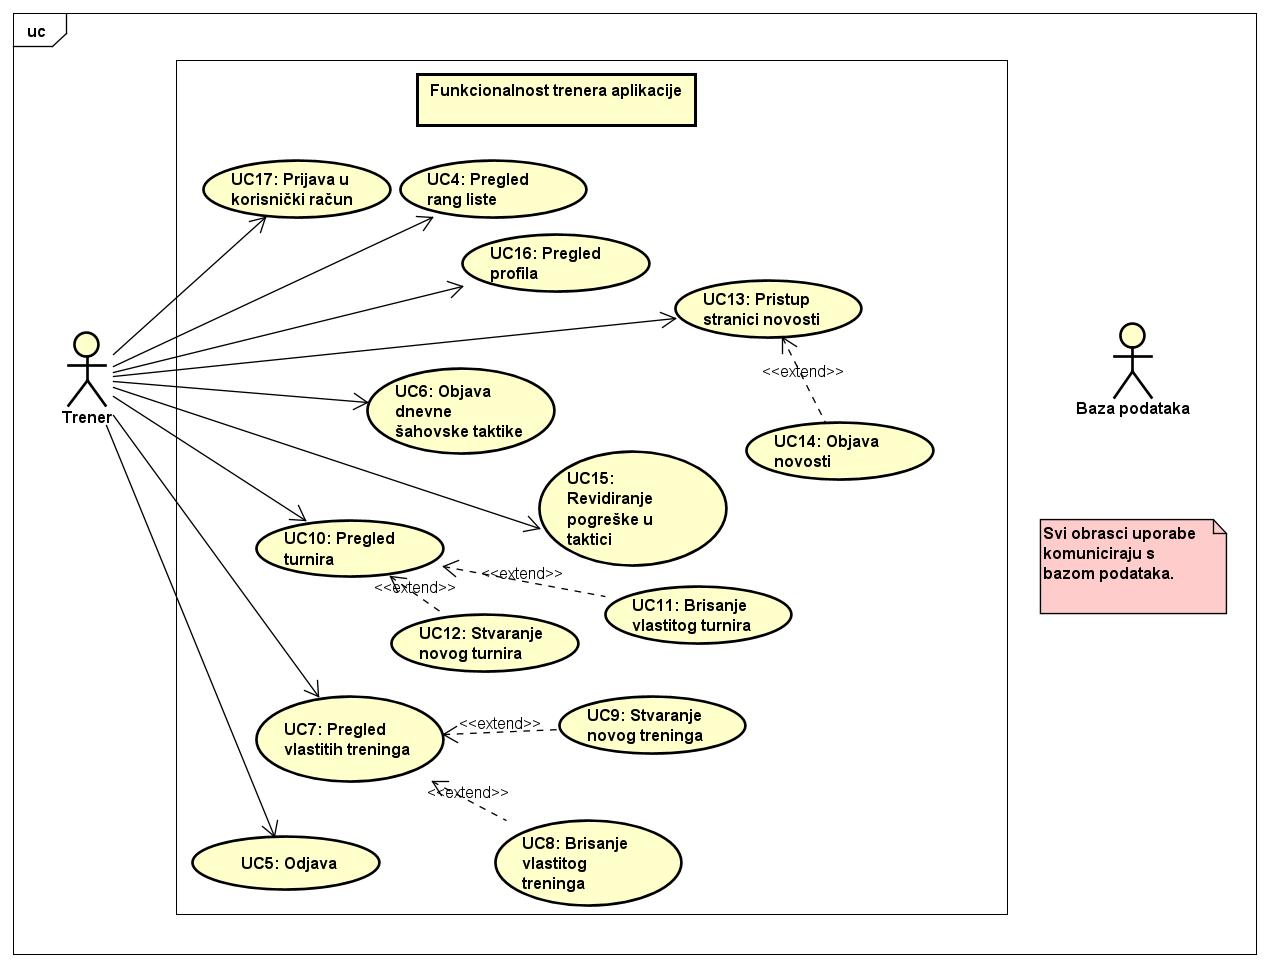
\includegraphics[scale=0.41]{dijagrami/UseCaseTrener.jpg} %veličina slike u odnosu na originalnu datoteku i pozicija slike
			\caption{Dijagram obrazaca uporabe za trenera}
			\label{fig:DOU_T}
		\end{figure}
		
		
		\begin{figure}[H]
			\centerfloat
			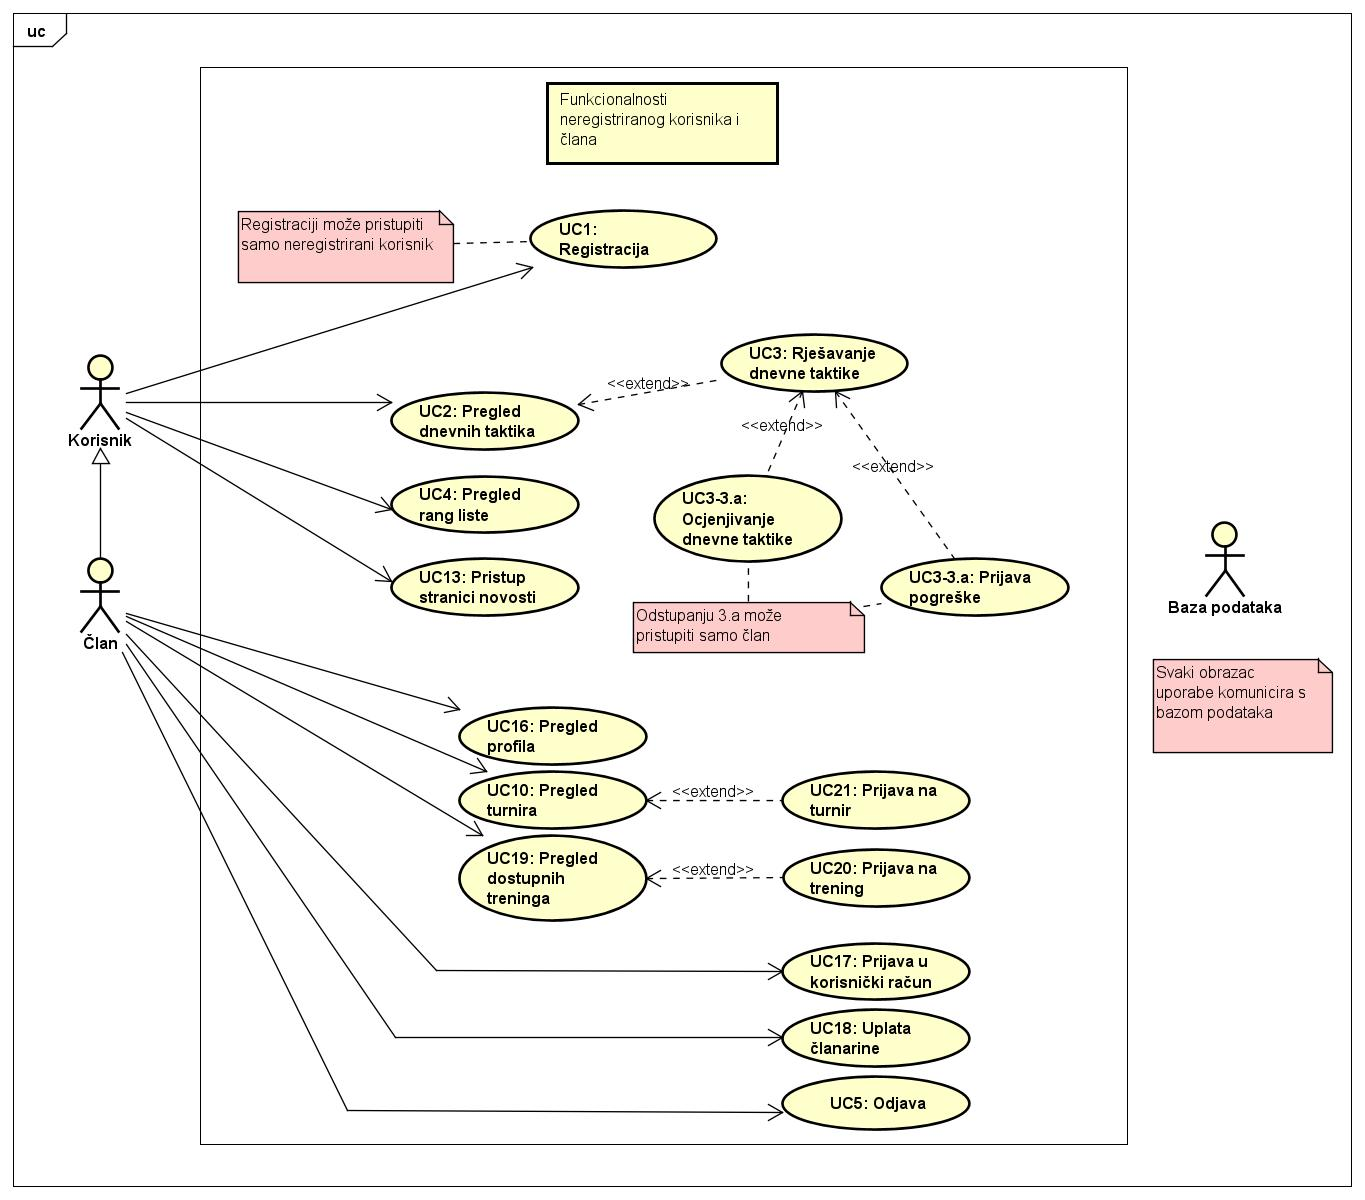
\includegraphics[scale=0.37]{dijagrami/UseCaseKorisnikClan.jpg} %veličina slike u odnosu na originalnu datoteku i pozicija slike
			\caption{Dijagram obrazaca uporabe za neregistriranog korisnika i člana}
			\label{fig:DOU_KC}
		\end{figure}
		
		
		\begin{figure}[H]
			\centerfloat
			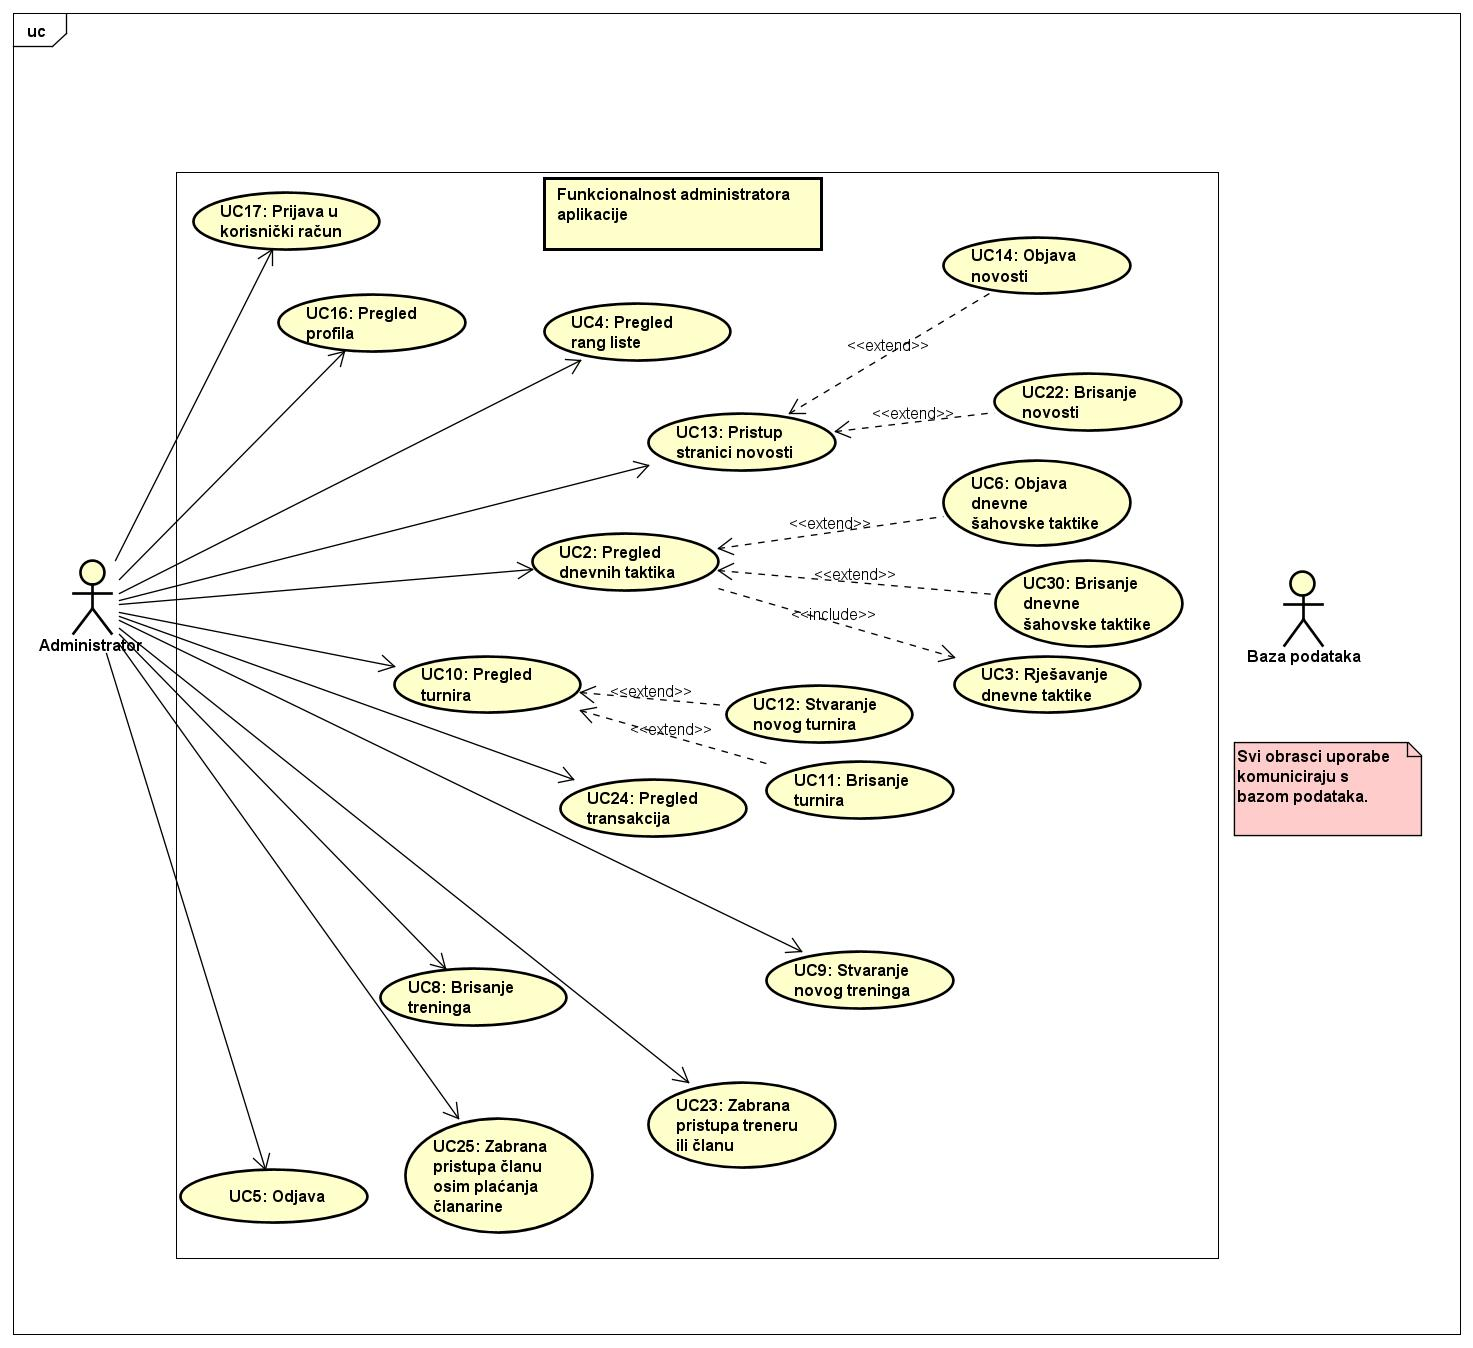
\includegraphics[scale=0.35]{dijagrami/UseCaseAdministrator.jpg} %veličina slike u odnosu na originalnu datoteku i pozicija slike
			\caption{Dijagram obrazaca uporabe za administratora}
			\label{fig:DOU_A}
		\end{figure}
		
		\eject
				
			\subsection{Sekvencijski dijagrami}
			
			
				\textbf{Obrazac uporabe UC9 - Stvaranje novog treninga}\\
				Trener šalje zahtjev web aplikaciji za stvaranje novog treninga. Web aplikacija dohvaća iz baze podataka sve ostale treninge tog trenera i provjerava da se novi trening ne preklapa ni s jednim postojećim treningom. Ako uistinu ne postoji preklapanje, novi trening se zapisuje u bazu podataka te se treneru šalje obavijest o uspjehu kreiranja novog treninga. Ako postoji preklapanje s već postojećim treningom, treneru web aplikacija javlja informacije o preklapanju i nemogućnosti stvaranja zatraženog treninga.
				\eject
				
				
				\begin{figure}[H]
					\centerfloat
        					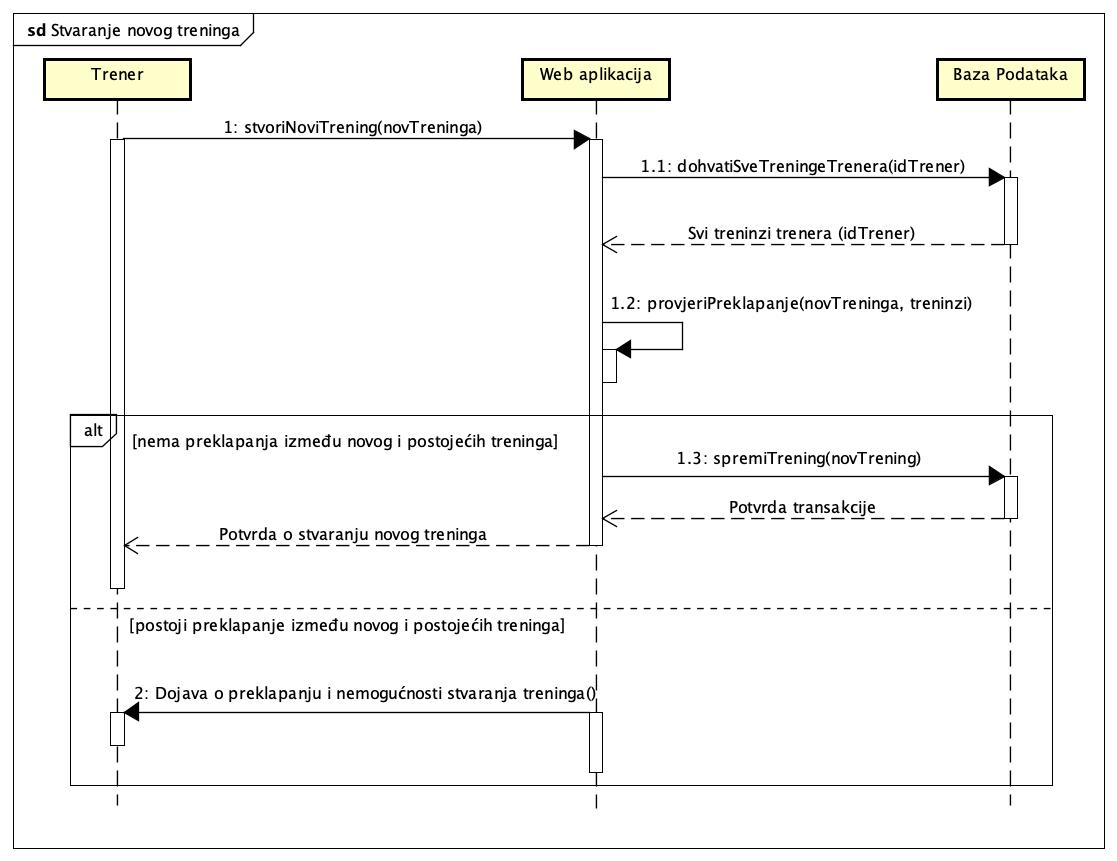
\includegraphics[scale=0.48]{dijagrami/StvaranjeNovogTreninga.jpg} %veličina slike u odnosu na originalnu datoteku i pozicija slike
        					\caption{Sekvencijski dijagram za UC9}
        					\label{fig:UC9}
				\end{figure}
				
				\eject
				
				\textbf{Obrazac uporabe UC15 - Revidiranje pogreške u taktici}\\
				\\Trener šalje zahtjev za prikaz određene dojave o pogrešci taktike kako bi ju mogao pobliže proučiti i odlučiti je li primjedba valjana. Poslužitelj zatraženu dojavu vadi iz baze podataka te ju prikazuje. Taj prikaz sastoji se od osnovnih informacija o dojavi poput ime prijavljene taktike, težine prijavljene taktike itd., ali se sastoji i od simulacije dvije šahovske ploče. Na prvoj ploča simulira se trenutni tijek taktike, a na drugoj se simulira novi tijek taktike koji je predložen u dojavi o pogrešci. Trener pritiskom na odgovarajuće gumbe šalje zahtjeve za sljedeći korak u simulaciji. Trener također može i poslati zahtjev za resetiranje simulacije i tako ju vratiti u početni položaj. Nakon što je proučio simulaciju trener šalje poslužitelju zahtjev za potvrdu ili odbacivanje dojave o pogrešci. Ako je trener potvrdio dojavu, poslužitelj ju tako mora obilježiti u bazi podataka, te zatim oduzeti odgovarajući broj bodova svim igračima koji su uspješno riješili 'zastarjelu' verziju taktike. Ako je trener odbacio dojavu, poslužitelj ju samo mora evidentirati kao odbačenu u bazi podataka.
			

				
				\begin{figure}[H]
					\centerfloat
        					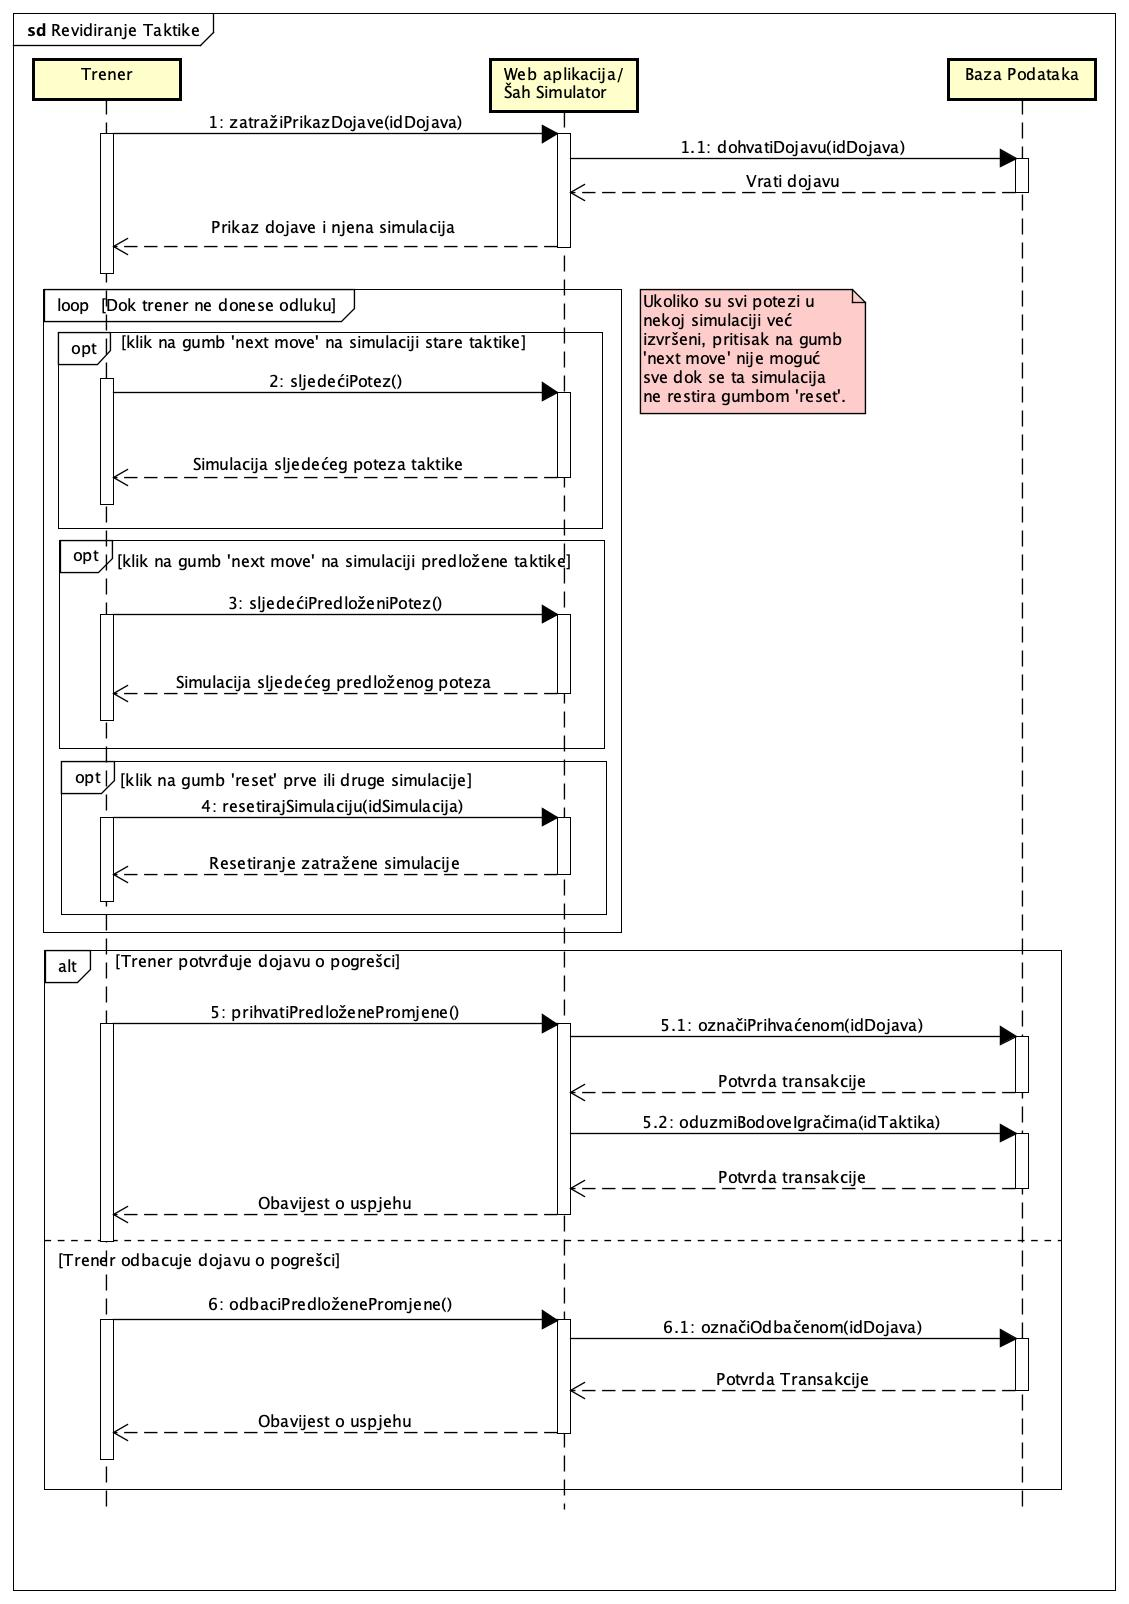
\includegraphics[scale=0.40]{dijagrami/RevidiranjeTaktike.jpg} %veličina slike u odnosu na originalnu datoteku i pozicija slike
        					\caption{Sekvencijski dijagram za UC15}
        					\label{fig:UC15}
				\end{figure}
				
				\eject
	
				\textbf{Obrazac uporabe UC6 - Objava taktike}\\
				\\Trener odabire kreaciju (objavu) nove taktike te mu web aplikacija vraća prikaz prazne ploče s figuricama sa strane. Trener zatim kreće s postavljanjem početnog stanja ploče. Mišem može povući željene figurice na njihovo mjesto te mu aplikacija to prikazuje. Postupak se ponavlja sve dok trener ne odluči da je početno stanje pripremljeno. To se javlja aplikaciji te se kreće u stanje rješavanja taktike. Trener odabire točne poteze bijelog i crnog igrača te se ti potezi prikazuju. Nakon što je unesen posljednji potez, trener zaključava unos poteza te objavljuje taktiku. Aplikacija šalje bazi podataka zahtjev za spremanjem taktike te prikazuje treneru poruku da je taktika objavljena.
			

				
				\begin{figure}[H]
					\centerfloat
					\advance\leftskip0.7cm
        					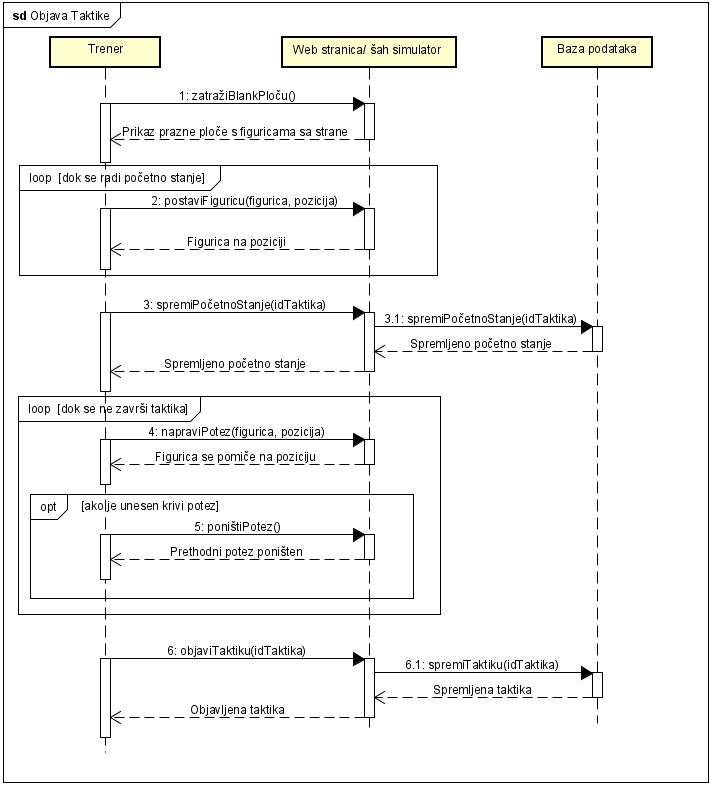
\includegraphics[scale=0.90]{dijagrami/ObjavaTaktike.jpg} %veličina slike u odnosu na originalnu datoteku i pozicija slike
        					\caption{Sekvencijski dijagram za UC6}
        					\label{fig:UC6}
				\end{figure}
				
				\eject
				
				\textbf{Obrazac uporabe UC3 - Rješavanje taktike}\\
				\\Korisnik otvara taktiku koja se dohvaća iz baze podataka. Korisnik zatim rješava tu taktiku te se pokreće tajmer. U slučaju krivog poteza, korisnik je obaviješten. Ako korisnik smatra da je taktika pogrešna, može spremiti svoju taktiku koja se šalje u bazu podataka. Nakon točnog rješavanja taktike, aplikacija računa postignute bodove na temelju vremena rješavanja i težine taktike. Bodovi zajedno s korisnikovim ID-om se spremaju u bazu podataka.
				\eject
				
				\begin{figure}[H]
					\centerfloat
					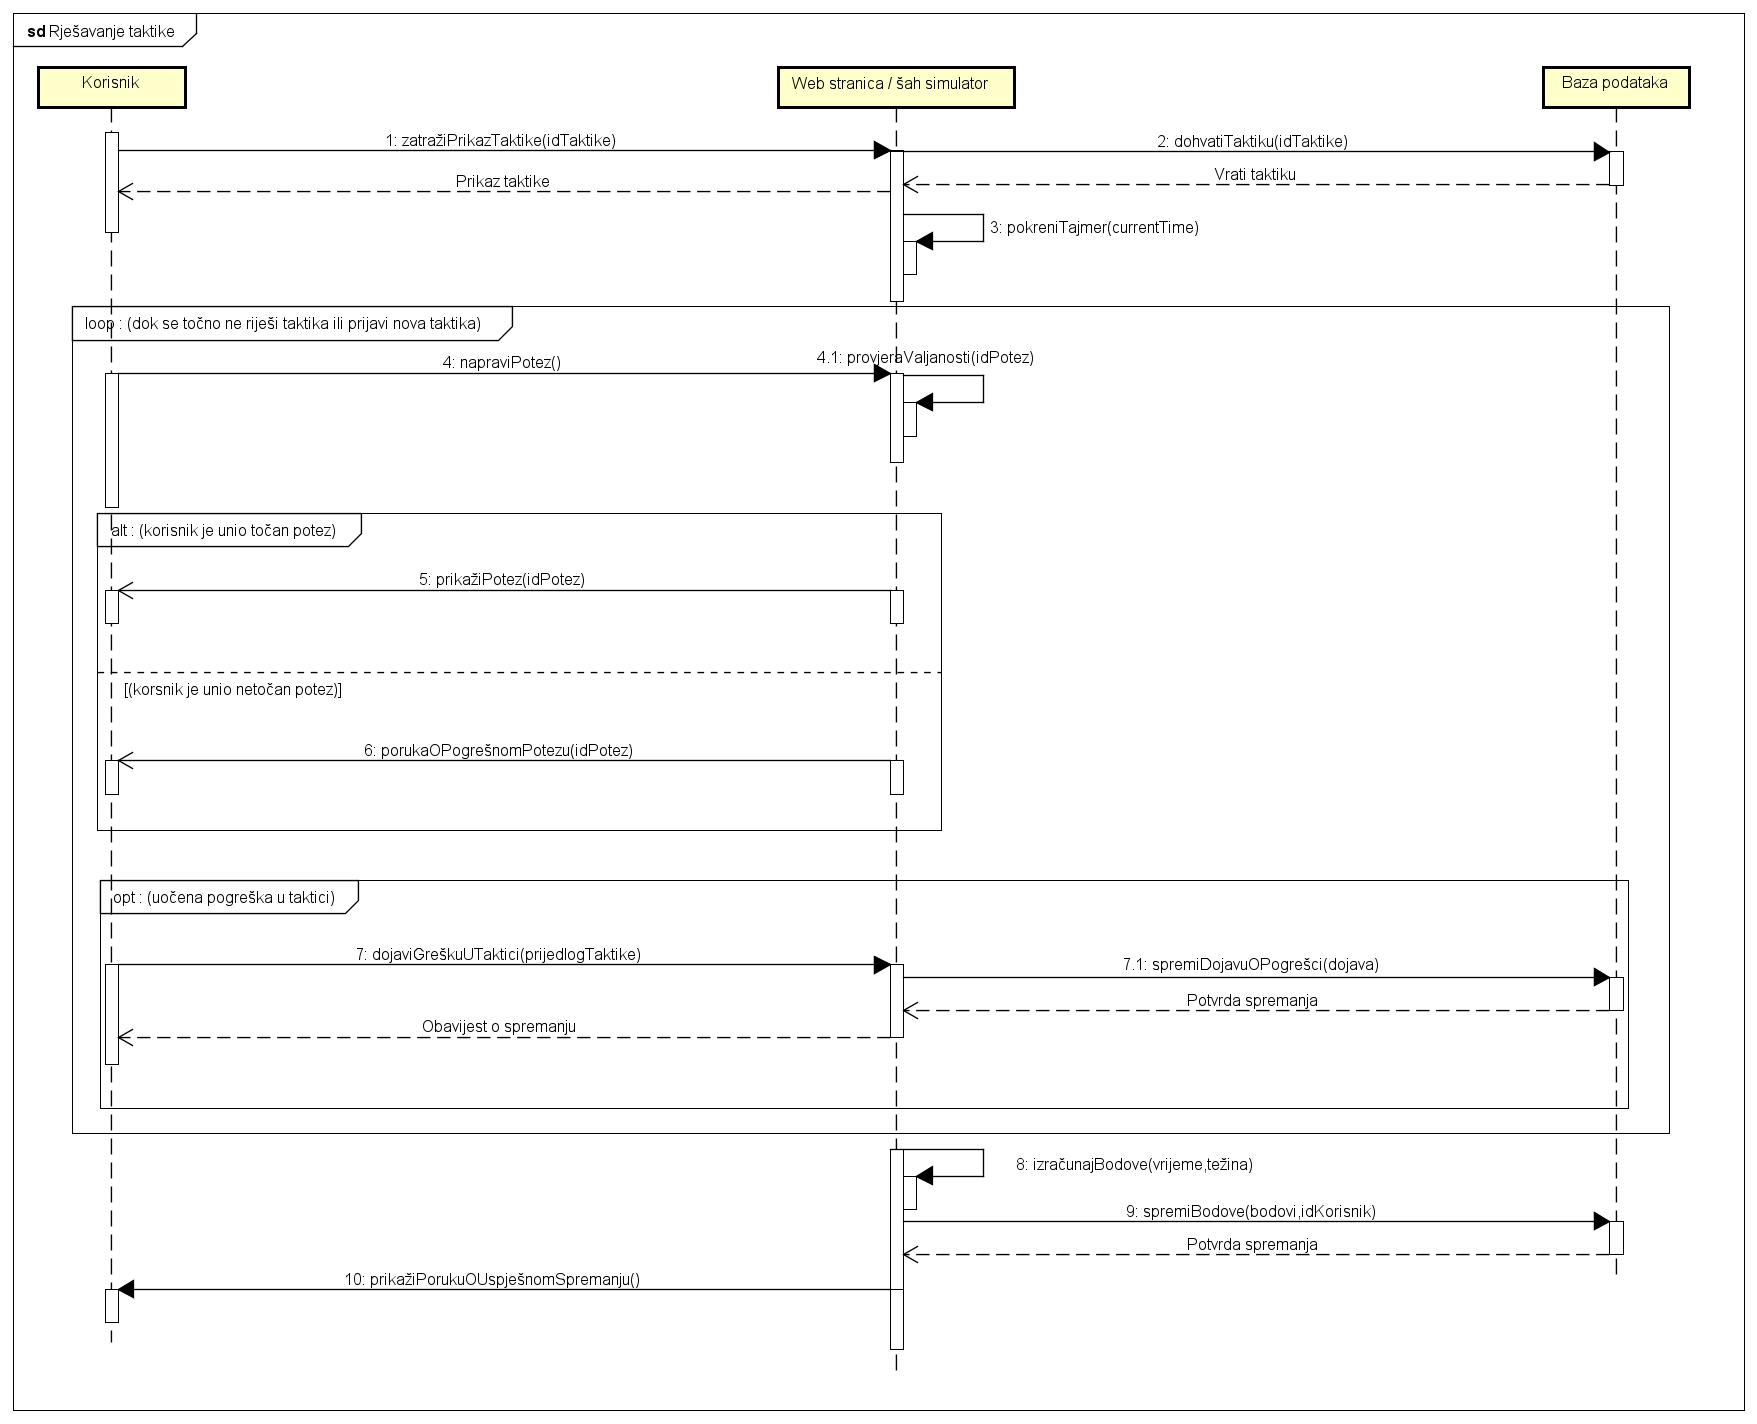
\includegraphics[scale=0.30]{dijagrami/RijesavanjeTaktike.jpg} %veličina slike u odnosu na originalnu datoteku i pozicija slike
					\caption{Sekvencijski dijagram za UC3}
					\label{fig:UC3}
				\end{figure}
				
				\eject

		\section{Ostali zahtjevi}
			
			Sustav mora osigurati da odgovor na svaki zahtjev dođe unutar 5 sekundi.  Sustav mora isto tako osiguravati da korisnici imaju sigurne šifre za svoje korisničke račune kako bi što bolje poboljšao sigurnost sustava. Sustav će koristiti protokol HTTP za komunikaciju između korisnika i servera. Sustav mora osigurati da svaka osoba ima samo jednu ulogu u aplikaciji. Sustav mora osigurati da korisnici ne mogu raditi ilegalne poteze u šahu.\\
			Sustav mora osigurati da korisnik mora unijeti sve potrebne podatke. \\
			Treneri prilikom stvaranja novog turnira mora unijeti naziv, datum i vrijeme početka te opis turnira. Treneri prilikom stvaranja novog termina treninga ne smije unijeti vrijeme koje mu je već zauzeto drugim terminom. Trener prilikom unosa nove novosti mora osigurati da novost ima naslov i sadržaj. \\
			Administrator prilikom stvaranja novog turnira mora unijeti naziv, datum i vrijeme početka, opis turnira te mora navesti trenera kojeg će sustav prepoznati kao organizatora turnira, pošto će tom treneru biti dane organizatorske ovlasti nad turnirom. Administrator prilikom stvaranja novog termina treninga mora navesti trenera kojem stvara termin te ne smije unijeti vrijeme koje je tom treneru već zauzeto drugim terminom.\\
			Član mora prilikom prijave pogreške u dnevnoj taktici mora unijeti poteze koje smatra ispravnim te opis tih poteza.\\
			Sustav mora mjeriti svakom članu vrijeme potrebno za rješavanje dnevne taktike te koristeći izmjereno vrijeme i ocjenu težine taktike dodijeliti članu bodove za tu taktiku. Sustav na bazi zbroja svih bodova, kreira težinsku listu rang listu članova.\\
			Korisničko sučelje će podržavati samo engleski jezik. Korisničko sučelje mora biti intuitivno za korištenje.\\
			
		 
			 
			 
			 
			 
	